\documentclass[../main.tex]{subfiles}
\graphicspath{
    {"../img/"}
    {"img/"}
}

\begin{document}
    \subsection{Sumowanie szeregów}
    \begin{figure}[h]
        \centering
        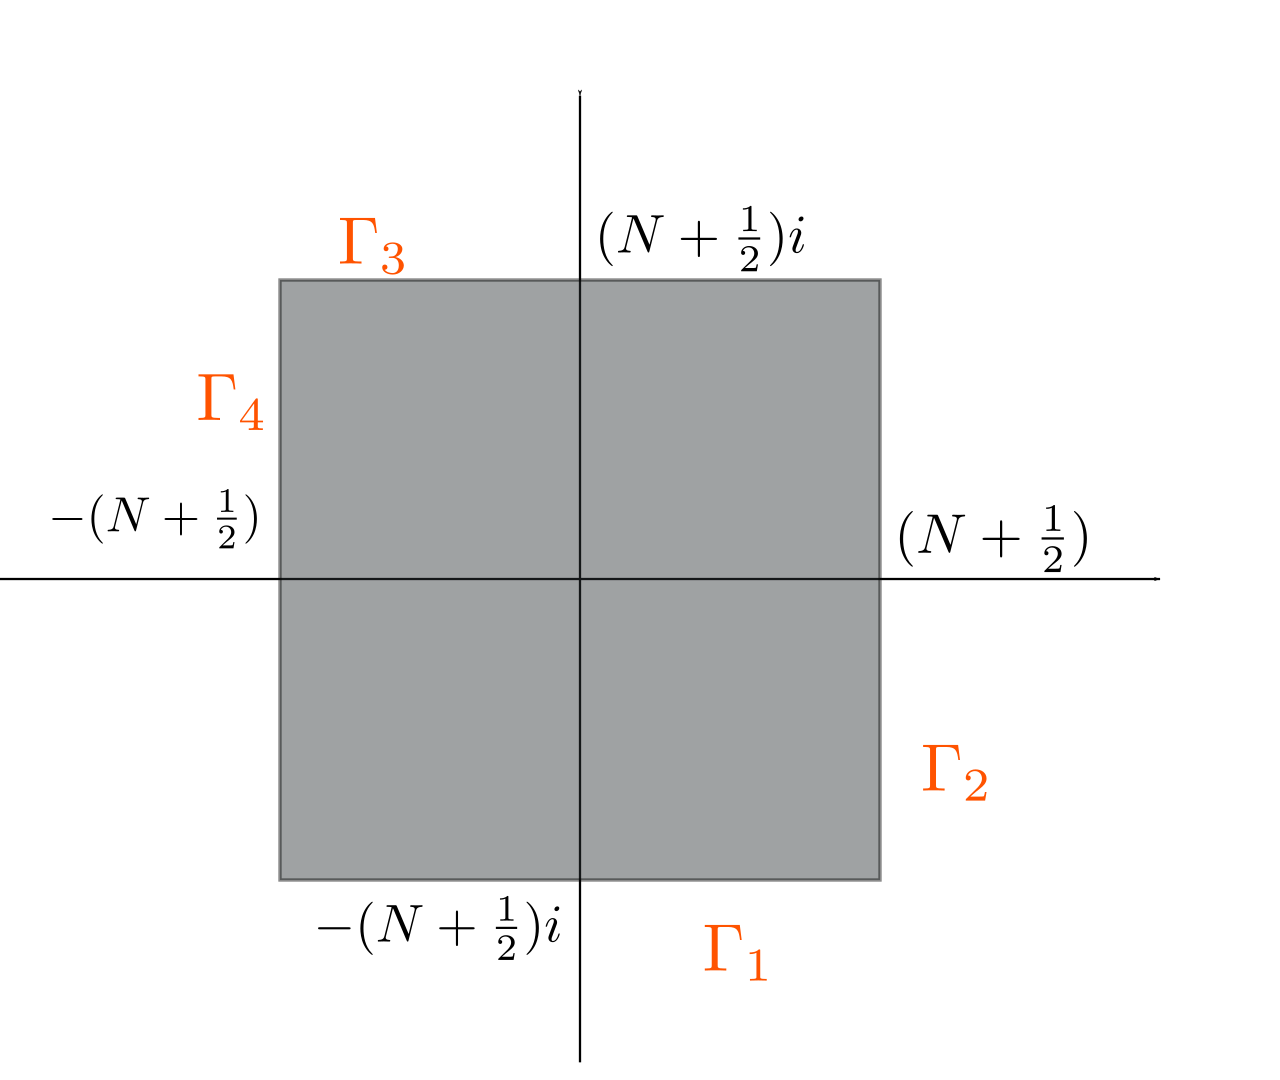
\includegraphics[width=0.8\textwidth]{w16-1}
        \caption{Kontur $\Gamma$}
        \label{fig:w16-1}
    \end{figure}
    \begin{stw}
        Niech $\Gamma$ - kontur przechodzący przez wierzchołki
        \[
            \left(N \pm \frac{1}{2}\right)\left(1 \pm i\right)\quad (\text{Rysunek }\ref{fig:w16-1})
        .\]
    I niech $f(z)$ - taka, że
        \[
            \underset{M}{\exists} \quad \underset{|z| > M}{\forall} \quad \left| f(z) \right| < \frac{const}{\left| z \right| ^2}
        ,\]
    $f(z)$ nie ma biegunów na $\Gamma$ oraz nie ma biegunów dla $z\in \mathbb{Z}$.
        Wówczas
        \[
            \lim\limits_{N\to\infty}\int\limits_{\Gamma}f(z) \ctg(\pi z)dz = 0
        .\]
    \end{stw}
    \begin{proof}
        Oszacujemy $\ctg(\pi z)$.\\
        Dla  $z\in \Gamma$
        \begin{enumerate}[a)]
            \item Jeżeli $z\in \Gamma_4$ lub $\Gamma_2$, to
                \[
                    \Gamma_2 = \left\{ y\in \left[ -N - \frac{1}{2}, N + \frac{1}{2} \right] , z = N + \frac{1}{2} + iy \right\}
                .\]
                \[
                    \Gamma_4 = \left\{ y\in \left[ -N - \frac{1}{2}, N + \frac{1}{2} \right] , z = -(N + \frac{1}{2}) + iy \right\}
                .\]
            \[
                \left| \ctg(\pi z) \right| = \left| \frac{e^{i\pi z} + e^{-i \pi z}}{e^{i \pi z} - e^{- i \pi z}} \right|\cdot \left| \frac{2i}{2} \right| = \left| \frac{e^{i\pi(N + \frac{1}{2} + iy)} + e^{-i\pi(N + \frac{1}{2} + iy)}}{e^{i\pi(N + \frac{1}{2} + iy)} - e^{-i\pi(N + \frac{1}{2} + iy)}} \right|
            .\]
        Dalej mamy dla $\left| e^{iN\pi} \right| = 1$
        \begin{equation}
            \label{eqn: delta}
            \left| \frac{e^{i\pi(N + \frac{1}{2})}\cdot e^{-y\pi} + e^{-i\pi(N + \frac{1}{2})}\cdot e^{y\pi}}{e^{i\pi(N + \frac{1}{2})}\cdot e^{-y\pi} - e^{-i\pi(N + \frac{1}{2})}\cdot e^{y\pi}} \right| \tag{$\Delta$}
        \end{equation}
    \textbf{Obserwacja: }
                \[
                    \lim\limits_{x\to +\infty} \frac{e^{x} + e^{-x}}{e^{x} - e^{-x}} = \lim\limits_{x\to + \infty} \frac{e^x(1+e^{-2x})}{e^{x}(1-e^{-2x})} = 1
                .\]
            Zatem
            \[
                \left|\eqref{eqn: delta}\right| \le \frac{2\left| e^{i\pi(N + \frac{1}{2})}\cdot e^{\pi N} \right|}{\left| e^{i\pi(N + \frac{1}{2})} \cdot e^{\pi(N+\frac{1}{2})} - e^{i \pi(N + \frac{1}{2})}\cdot e^{\pi(N + \frac{1}{2})} \right| } \le \frac{2 \left| e^{i\pi(N + \frac{1}{2})} \right|}{\left| e^{i \pi(N + \frac{1}{2})} \cdot e^{-2\pi(N + \frac{1}{2})} + e^{i\pi(N + \frac{1}{2})} \right| } < \text{const}
            .\]
    \item Analogicznie pokażemy, że $\ctg(\pi z)$ jest ograniczony dla $z\in \Gamma_4, \Gamma_1, \Gamma_3$. Zatem
        \[
            \left| \int\limits_{\Gamma}f(z)\ctg(\pi z)dz \right| \le \left| \underset{z\in\Gamma}{\max}f(z)  \right| \cdot \left| 8N + 4 \right| \cdot \text{const} \underset{N > M}{\le} \frac{\text{const}}{N^2} (8N + 4) \cdot \text{const} \underset{N \to + \infty}{\longrightarrow}  0
        .\]
        \end{enumerate}
    \end{proof}
    \textbf{Wniosek:}\\
    Niech $b$ - zbiór wszystkich biegunów $f(z)\ctg(\pi z)$
    \[
        0 = \lim\limits_{N\to \infty} \int\limits_{\Gamma}f(z) \ctg(\pi z)dz = 2\pi i \sum_b \Res\left( f(z) \ctg(\pi z) \right) = 0
    .\]
\begin{pytanie}
    W jakich punktach $\ctg(\pi z)$ ma bieguny i którego rzędu?
\end{pytanie}
Zauważmy, że
\[
    \frac{(\pi z-0 \pi)\cos(\pi z)}{\pi\sin(\pi z)} \underset{z\to 0}{\longrightarrow} \frac{1}{\pi}
.\]
A np.
\[
    \lim\limits_{z\to n}\frac{(z-n)\cos(\pi z)}{\sin(\pi z)} \overset{H}{=} \lim\limits_{z\to n} \frac{\cos(\pi z) - (z-n)\pi \sin(\pi z)}{\pi \cos(\pi z)} \underset{z\to n}{\longrightarrow} \frac{1}{\pi}
.\]
Wiemy, że
\[
    \sum_b \Res f(z) \ctg(\pi z) = 0
,\]
czyli
\[
    0 = \sum_c \Res f(z) \ctg(\pi z) + \sum_d \Res f(z) \ctg(\pi z)
.\]
gdzie $c$ - bieguny $\ctg(\pi z)$, $d$ - bieguny $f(z)$. Zatem
\[
    \frac{1}{\pi} \sum_{n=-\infty}^{+\infty} f(n) = - \sum_d \Res f(z) \ctg(\pi z)
.\]
\begin{przyklad}
    \[
    \sum_{n=1}^{\infty} \frac{1}{n^2} = \quad ?
    \]
    Wiemy, że
    \[
        \sum_b \Res f(z) \ctg(\pi z) = 0
    .\]
\[
    f(z) = \frac{1}{z^2}
.\]
Rozdzielmy sobie sumę na dwie:
    \[
        \underbrace{\sum_{n=1}^{\infty} \frac{1}{\pi}f(n) + \sum_{n=-1}^{-\infty} \frac{1}{\pi}f(n)}_{\text{bieguny }\ctg(\pi z) \text{ bez }0} + \quad\underset{z = 0}{\Res}\quad  f(z) \ctg(\pi z) = 0
    .\]
\[
    \sum_{n=1}^{\infty} \frac{1}{\pi} n^2 + \sum_{n=-1}^{-\infty} \frac{1}{\pi}\left( \frac{1}{n^2} \right) = -\quad \underset{z=0}{\Res}\quad f(z) \ctg(\pi z)
.\]
\[
    \sum_{n=1}^{\infty} \frac{1}{n^2} = - \frac{\pi}{2} \quad\underset{z = 0}{\Res}\quad \frac{\ctg(\pi z)}{z^2}
.\]
\end{przyklad}
\textbf{Obserwacja:} Niech $P = \left\{ z\in \Omega, f(z) = 0 \right\}$. Niech $D$ - zbiór biegunów $f(z)$ na $\Omega$ i $f$ - holomorficzna na $\Omega - D$. Wówczas $\frac{f'}{f}$ ma na $\Omega$ bieguny pierwszego rzędu dla $z \in P \cup D$

\begin{proof}
    Niech $z_0\in P$. Oznacza to, że
    \[
        f(z) = a_k (z-z_0)^k + a_{k+1} (z-z_0)^{k+1} + \ldots
    ,\]
gdzie $k \ge 1$. Wówczas
\[
    \frac{f'(z)}{f(z)} = \frac{ka_k(z-z_0)^{k-1} + (k+1)a_{k+1}(z-z_0)^k + \ldots}{a_k(z-z_0)^k + a_{k+1}(z-z_0)^{k+1} + \ldots} =
\]
\[
    = \frac{1}{z-z_0}\cdot \frac{ka_k + (k+1)a_{k+1}(z-z_0) + \ldots}{a_k + a_{k+ 1}(z-z_0) + \ldots}
.\]
\[
    \lim\limits_{z\to z_0} \frac{(z-z_0)f'}{f} = k
.\]
Czyli $\frac{f'}{f}$ ma w $z_0\in P$ biegun pierwszego rzędu i wynosi $k$.
\end{proof}
Niech $z_1\in D$, $f$ ma w $z = z_1$ biegun $n$ - tego rzędu. Oznacza to, że
\[
    f(z) = \frac{a_{-n}}{(z-z_1)^n} + \frac{a_{-(n-1)}}{(z-z_1)^{n-1}} + \ldots
.\]
Wówczas
\[
    \frac{f'(z)}{f(z)} = \frac{\frac{-na_{-n}}{(z-z_1)^{n+1}} + \frac{-(n-1)a_{-(n-1)}}{(z-z_1)^n} + \ldots }{\frac{a_{-n}}{(z-z_1)^n} + \frac{a_{-(n-1)}}{(z-z_1)^{n-1}} + \ldots} = \frac{1}{(z-z_1)}\frac{\left[ -na_{-n} + -(n-1)a_{-(n-1)}(z-z_1) + \ldots \right] }{\left[ a_{-n} + a_{-(n-1)}(z-z_1) + \ldots \right] }
.\]
\[
    \lim\limits_{z\to z_n}\frac{f'}{f} (z-z_1) = -n
.\]
\textbf{Wniosek:}
\[
    \frac{1}{2\pi i}\int\limits_{\partial \Omega}\frac{f'}{f} = \sum_{z\in D} \frac{f'}{f} + \sum_{z_1\in P} \frac{f'}{f}
.\]
\end{document}
